\documentclass[11pt,a4paper]{article}
\usepackage[T1]{fontenc}
\usepackage[utf8]{inputenc}
\usepackage{lmodern}
\usepackage{amsmath,amssymb}
\usepackage{booktabs}
\usepackage{geometry}
\usepackage{hyperref}
\usepackage{enumitem}
\usepackage{xcolor}
\usepackage{graphicx}

\geometry{margin=2.2cm}
\graphicspath{{../slides/figures/}}

\definecolor{linkgreen}{RGB}{22,101,52}
\hypersetup{colorlinks=true,linkcolor=linkgreen,urlcolor=linkgreen}

\title{Hospital Chatbot for Color Coded Clinical Pathways\\Speaker Guide}
\author{Quaigraine Samuel \and Twum Samuel\\Department of Mathematics, KNUST}
\date{August 2026}

\begin{document}
\maketitle
\tableofcontents
\newpage

\section{Overview}

\textbf{Title:} Hospital Chatbot for Color Coded Clinical Pathways

\textbf{Template:} KNUST Beamer (Gabby.sty)

\textbf{Duration:} 20--30 minutes plus questions.

\textbf{Full step-by-step script:} see \texttt{presenter-walkthrough.pdf} (companion handbook with ON SCREEN / SAY THIS boxes for all 20 slides).

\textbf{Core message:} Patients present unstructured text $X$ while vitals $\mathbf{v}$ are often unknown. The protocol still requires $\hat{c}$ and $C = f_{\mathrm{SATS}}(\hat{c})$ before TEWS. The chatbot also binds $C$ to pathway $P(C)$ and reduces acute-zone load (transshipment LP).

\textbf{Key numbers:}
\begin{itemize}[noitemsep]
  \item N=1000, skewed mix 5\% / 15\% / 30\% / 25\% / 25\%
  \item Colour accuracy: 97.5\% (975/1000)
  \item Level 1 recall: 94.0\% (47/50)
  \item Green diversion: 500 patients (50\%)
  \item Transshipment: cost 7150 $\to$ 2700 (62\% reduction); acute load 900 $\to$ 500 (44\%)
\end{itemize}

\section{Section 1: Research gaps (2 slides)}

\subsection{ED overcrowding and waiting for care}

Two-column image slide before the gap list:
\begin{itemize}[noitemsep]
  \item \textbf{Image 1:} queue for care (Longdon, 2026, Citi Newsroom).
  \item \textbf{Image 2:} Korle-Bu overcrowding fact-check (Aminu, 2021, Ghana Fact).
\end{itemize}
Sources appear as tiny URLs under each image on the slide.

\subsection{Research gaps in prior work}

\textbf{Say:} We aim to infer acuity from free-form chief complaints to reduce ED overcrowding and waiting times (Mitchell et al., 2023; Yilmaz, 2021). Each gap is one cited sentence from prior literature---not our project features.

Walk all five items and name the references on slide:
\begin{enumerate}[noitemsep]
  \item Vitals-first bias --- SATS2012, Rominski et al. 2014, Stewart et al. 2023.
  \item Pathway discontinuity --- Nurchis et al. 2025, Sundstr{\"o}m et al. 2014.
  \item Overcrowding without text pre-triage --- Yilmaz 2021, Mitchell et al. 2023.
  \item Generative vs constrained NLP --- Stewart et al. 2023, Cheng et al. 2025.
  \item Class imbalance --- Stewart et al. 2023, Berkowitz et al. 2019.
\end{enumerate}

Image-only gap slide removed. Own case-study numbers cite as \textbf{(This study, 2026)} on slides.

\section{Section 2: Community Hospital (7 slides)}

\subsection{Acuity chart}

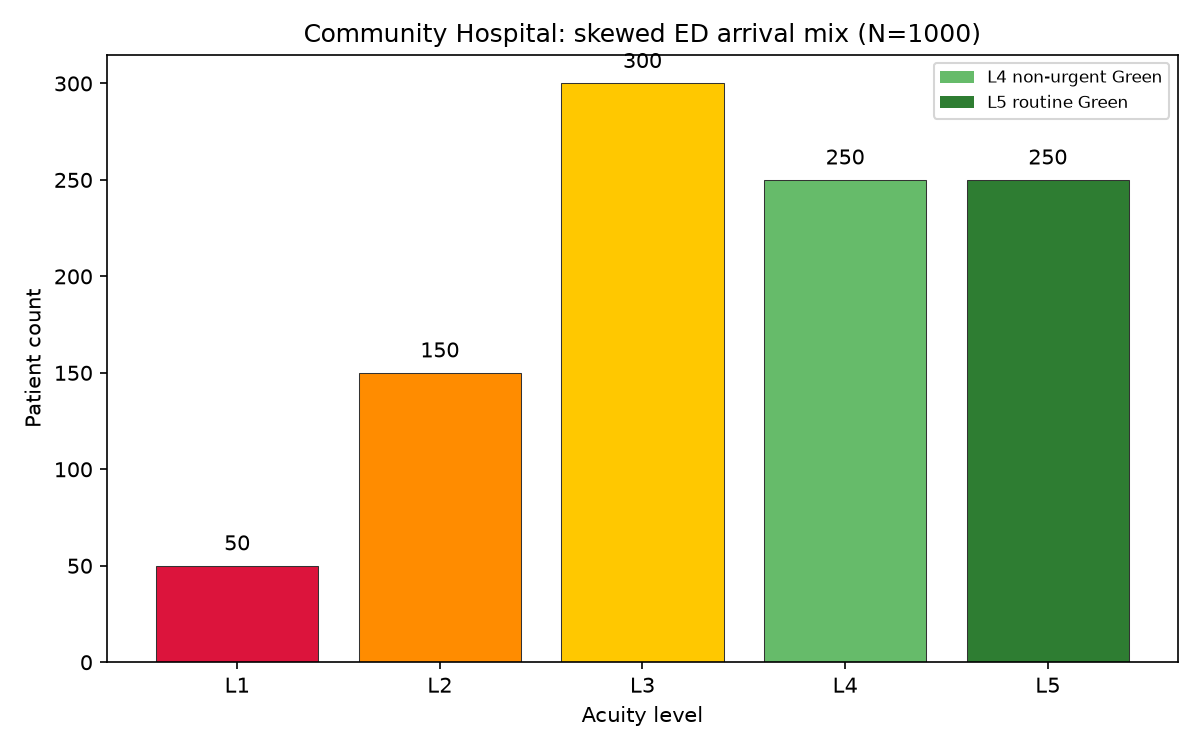
\includegraphics[width=0.75\textwidth]{acuity_distribution.png}

\textbf{Say:} Skewed mix, not balanced. L4 and L5 bars are different shades; both map to SATS Green.

\subsection{Accuracy chart}

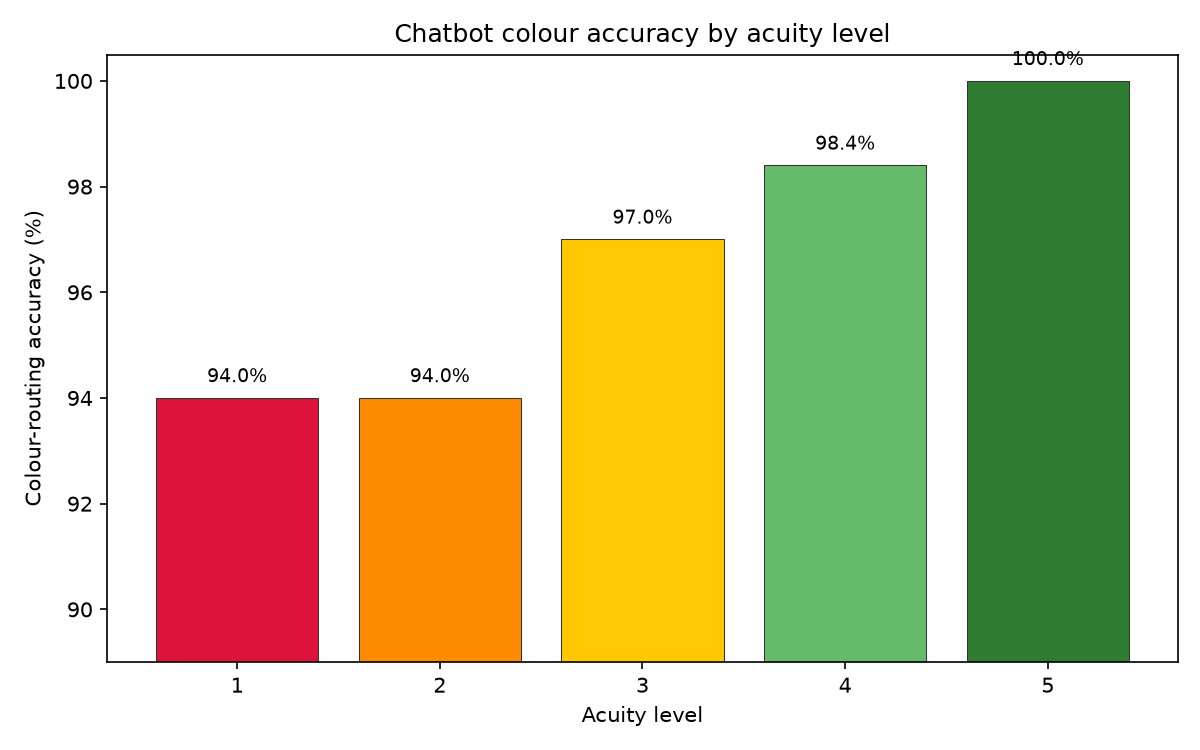
\includegraphics[width=0.75\textwidth]{chatbot_accuracy_by_level.png}

\textbf{Say:} 97.5\% overall. Errors on adjacent levels and borderline cases (~7\% of rows flagged).

\section{Section 3: Transshipment (4 slides)}

\textbf{Supplies:} (50, 150, 300, 500). \textbf{Demands:} resus 50, majors 450, OPD 500.

Without chatbot: Green mis-routes to majors (acute load 900). With chatbot: flow 4$\to$5$\to$9 (acute load 500).

Network diagram: layer labels (Sources, Transshipment, Destinations) sit left of the node boxes. ``Why transshipment fits triage'' slide removed.

\section{Section 4: NLP design (2 slides)}

Fixed outputs: $\hat{c}$, $C$, $P(C)$. Contrast with generative LLMs (comparison table). BioBERT pipeline and future fusion slides removed; fusion remains in \texttt{triage-fusion/} documentation.

\section{Section 5: Conclusion (2 slides)}

\textbf{Summary:} four numbered takeaways (gaps, case study, transshipment, NLP design).

\textbf{Limitations only:} synthetic cohort, simulated eval, analytical transshipment model. No ``next steps'' slide.

\textbf{References slide:} final frame lists full bibliography (\texttt{references.bib}); compile with \texttt{bibtex main}.

\section{Anticipated Q\&A}

\begin{description}[style=nextline]
  \item[Why synthetic data?] Skewed mix teaches realistic ED statistics; 8k holdout validates the model separately.
  \item[Why not ChatGPT?] Bounded output; no hallucinated urgency.
  \item[Why two greens on chart?] L4 non-urgent vs L5 routine; same SATS colour, different acuity levels.
  \item[Is TEWS included?] Not yet; see \texttt{triage-fusion/}.
\end{description}

\section{Rebuild}

\begin{verbatim}
python3 community-hospital/scripts/generate_synthetic_data.py
python3 community-hospital/scripts/run_chatbot_eval.py
community-hospital/.venv/bin/python community-hospital/scripts/transshipment_ed.py
community-hospital/.venv/bin/python community-hospital/scripts/analyze_case_study.py
cp community-hospital/analysis/figures/*.png community-hospital/slides/figures/
cd community-hospital/slides
pdflatex main.tex && bibtex main && pdflatex main.tex && pdflatex main.tex
cd ../guide && pdflatex presentation-guide.tex && pdflatex presentation-guide.tex
pdflatex presenter-walkthrough.tex && pdflatex presenter-walkthrough.tex
\end{verbatim}

\end{document}
